\documentclass[11pt,a4paper]{article}
%-------------------------------------------
%---Packages--------------------------------
%-------------------------------------------
\usepackage[utf8]{inputenc}
%\usepackage[T1]{fontenc}
%\usepackage{txfonts}
\usepackage{amsmath}
\usepackage{amsthm}
\usepackage{amsfonts}
\usepackage{array}
\usepackage{amssymb}
\usepackage{blindtext}
\usepackage{caption}
\usepackage{color}
\usepackage{csquotes}	    %
\usepackage{enumitem}	    %pour mieux bosser avec les listes. ajoute option label
\usepackage[yyyymmdd]{datetime}        %pour définir date custom
\usepackage{etaremune}
\usepackage{environ}
\usepackage{fancybox}
\usepackage{fancyhdr} 	    % Custom headers and footers
\usepackage{fancyref}
%\usepackage{float}
\usepackage{floatrow}       %float and floatrow can't be together...
\usepackage{gensymb}
\usepackage{graphicx}
\usepackage[colorlinks=true, linkcolor=purple, citecolor=cyan]{hyperref}
\usepackage{footnotebackref}
\usepackage{lipsum}
\usepackage{mathtools}
\usepackage{multicol}	    %gérer plusieurs colonnes
\usepackage{setspace}
\usepackage{subcaption}
\usepackage{todonotes}	    %Bonne gestion des TODOs
%TODO commenté pour tester l'utilité... à voir% \usepackage[tc]{titlepic}      %Permet de mettre une image en page de garde
\usepackage{tikz}	    % Pour outil de dessin puissant
\usepackage{ulem}	    %underline sur plusieurs lignes (avec \uline{})
\usepackage{vmargin} 	    %gestion des marges, avec dans l'ordre : gauche, haut, droit, bas, en-tête, entre en-tête et texte, bas de page, hauteur entre bas de page et texte
\usepackage{wrapfig}
\usepackage{xcolor}
\usepackage{xparse}                    %Pour utiliser NewDocumentCommand et des arguments 'mmooo'
%\usepackage{fullpage} 	    %supprime toutes les marges allouées aux notes, aussi en haut et en bas

%\ExplSyntaxOn
\pagestyle{fancyplain}	    %Makes all pages in the document conform to the custom headers and footers

%-------------------------------------------
%---Document Commands-----------------------
%---------------------------{----------------
\NewDocumentCommand{\framecolorbox}{oommm}
 {% #1 = width (optional)
  % #2 = inner alignment (optional)
  % #3 = frame color
  % #4 = background color
  % #5 = text
  \IfValueTF{#1}%
   {\IfValueTF{#2}%
    {\fcolorbox{#3}{#4}{\makebox[#1][#2]{#5}}}%
    {\fcolorbox{#3}{#4}{\makebox[#1]{#5}}}%
   }%
   {\fcolorbox{#3}{#4}{#5}}%
 }%
%------------------------------------------------
%------------------ENGLISH----------------------
%----------------------------------------------

\NewDocumentCommand{\epflTitle}{mO{Olivier Cloux}O{\today}O{Notes de Cours en}D<>{../../Common}}%Arguments : Matière, Auteur, Date, Titre du doc
{
\begin{titlepage}
    \vspace*{\fill}
    \begin{center}
        \normalfont \normalsize
        \textsc{Ecole Polytechnique Fédérale de Lausanne} \\ [25pt] % Your university, school and/or department name(s)
        \textsc{#4} %Titre du doc
        \\ [0.4 pt]
        \horrule{0.5pt} \\[0.4cm] % Thin top horizontal rule
        \huge #1 \\ % Matière
        \horrule{2pt} \\[0.5cm] % Thick bottom horizontal rule
        
\includegraphics[width=8cm]{#5/EPFL_logo}
        ~\\[0.5 cm]
        \small\textsc{#2}\\[0.4cm]
        \small\textsc{#3}\\
        ~\\
        ~\\
        
\includegraphics[scale=0.5]{#5/creativeCommons}
    \end{center}
    \vspace*{\fill}
\end{titlepage}
}


%-------------------------------------------
%-------------MATH NEW COMMANDS-------------
%-------------------------------------------
\newcommand{\somme}[2]{\ensuremath{\sum\limits_{#2}^{#1}}}
\newcommand{\produit}[2]{\ensuremath{\prod\limits_{#2}^{#1}}}
\newcommand{\limite}{\lim\limits_}
\newcommand{\llimite}[3]{\limite{\substack{#1 \\ #2}}\left(#3\right)}	%limites à deux condiitons
\newcommand{\et}{\mbox{ et }}
\newcommand{\deriv}[1]{\ensuremath{\, \mathrm d #1}}	%sigle dx, dt,dy... des dérivées/intégrales
%\newcommand{\fx}{\ensuremath{f'(\textbf{x}_0 + h}}
\newcommand{\ninf}{\ensuremath{n \to \infty}}	       %pour les limites : n tend vers l'infini
\newcommand{\xinf}{\ensuremath{x \to \infty}}	       %pour les limites : x tend vers l'infini
\newcommand{\infint}{\ensuremath{\int_{-\infty}^{\infty}}}
\newcommand{\xo}{\ensuremath{x \to 0}}									%x to 0
\newcommand{\no}{\ensuremath{n \to 0}}									%n zéro
\newcommand{\xx}{\ensuremath{x \to x}}									%x to x
\newcommand{\Xo}{\ensuremath{x_0}}										%x zéro
\newcommand{\X}{\ensuremath{\mathbf{X}} }
\newcommand{\A}{\ensuremath{\mathbf{A}} }
\newcommand{\R}{\ensuremath{\mathbb{R}} }								%ensemble de R
\newcommand{\rn}{\ensuremath{\mathbb{R}^n} } 							%ensemble de R de taille n
\newcommand{\Rm}{\ensuremath{\mathbb{R}^m} }  							%ensemble de R de taille m
\newcommand{\C}{\ensuremath{\mathbb{C}} }
\newcommand{\N}{\ensuremath{\mathbb{N}} }
\newcommand{\Z}{\ensuremath{\mathbb{Z}} }
\newcommand{\Q}{\ensuremath{\mathbb{Q}} }
\newcommand{\rtor}{\ensuremath{\R \to \R} }
\newcommand{\pour}{\mbox{ pour }}
\newcommand{\coss}[1]{\ensuremath{\cos\(#1\)}}						%cosinus avec des parenthèses de bonne taille (genre frac)
\newcommand{\sinn}[1]{\ensuremath{\sin\(#1\)}}					%sinus avec des parentèses de bonne taille (genre frac)
\newcommand{\txtfrac}[2]{\ensuremath{\frac{\text{#1}}{\text{#2}}}}		%Fractions composées de texte
\newcommand{\evalfrac}[3]{\ensuremath{\left.\frac{#1}{#2}\right|_{#3}}}
\renewcommand{\(}{\left(}												%Parenthèse gauche de taille adaptive
\renewcommand{\)}{\right)}
\newcommand{\longeq}{=\joinrel=}												%Parenthèse droite de taille adaptive


%-------------------------------------------------------
%------------------MISC NEW COMMANDS--------------------
%-------------------------------------------------------
\newcommand{\degre}{\ensuremath{^\circ}}
%\newdateformat{\eudate}{\THEYEAR-\twodigit{\THEMONTH}-\twodigit{\THEDAY}}



%-------------------------------------------------------
%------------------TEXT NEW COMMANDS--------------------
%-------------------------------------------------------
\newcommand{\ts}{\textsuperscript}
\newcommand{\evid}[1]{\textbf{\uline{#1}}}        %mise en évidence (gras + souligné)



%\newcommand{\Exemple}{\underline{Exemple}}
\newcommand{\Theoreme}{\underline{Théorème}}
\newcommand{\Remarque}{\underline{Remarque}}
\newcommand{\Definition}{\underline{Définition} }
\newcommand{\skinf}{\sum^{\infty}_{k=0}}
\newcommand{\combi}[2]{\ensuremath{\begin{pmatrix} #1 \\ #2 \end{pmatrix}}}	%combinaison parmi 1 de 2
\newcommand{\intx}[3]{\ensuremath{\int_{#1}^{#2} #3 \deriv{x}}}				%intégrale dx
\newcommand{\intt}[3]{\ensuremath{\int_{#1}^{#2} #3 \deriv{t}}}				%intégrale dy
\newcommand{\misenforme}{\begin{center} Mis en forme jusqu'ici\\ \line(1,0){400}\\ normalement juste, mais à améliorer depuis ici\end{center}}	%raccourci pour mise en forme
\newcommand*\circled[1]{\tikz[baseline=(char.base)]{
            \node[shape=circle,draw,inner sep=1pt] (char) {#1};}}			%pour entourer un chiffre
\newcommand{\horrule}[1]{\rule{\linewidth}{#1}} 				% Create horizontal rule command with 1 argument of height

\theoremstyle{definition}
\newtheorem{exemp}{Exemple}
\newtheorem{examp}{Example}


%-------------------------------------------
%---Environments----------------------------
%-------------------------------------------
\NewEnviron{boite}[1][0.9]{%
	\begin{center}
		\framecolorbox{red}{white}{%
			\begin{minipage}{#1\textwidth}
 	 			\BODY
			\end{minipage}
		}
	\end{center}
}
\NewEnviron{blackbox}[1][0.9]{%
	\begin{center}
		\framecolorbox{black}{white}{%
			\begin{minipage}{#1\textwidth}
 	 			\BODY
			\end{minipage}
		}
	\end{center}
}
\NewEnviron{exemple}[1][0.8]{%
    \begin{center}
        \framecolorbox{white}{gray!20}{%
            \begin{minipage}{#1\textwidth}
                \begin{exemp}
                    \BODY
                \end{exemp}
            \end{minipage}
        }
    \end{center}
}
\NewEnviron{suiteExemple}[1][0.8]{%
    \begin{center}
        \framecolorbox{white}{gray!20}{%
            \begin{minipage}{#1\textwidth}
                \BODY
            \end{minipage}
        }
    \end{center}
}
\NewEnviron{colExemple}[1][0.8]{%
    \begin{center}
        \framecolorbox{white}{gray!20}{%
            \begin{minipage}{#1\columnwidth}
                \begin{exemp}
                    \BODY
                \end{exemp}
            \end{minipage}
        }
    \end{center}
}
\NewEnviron{example}[1][0.8]{%
    \begin{center}
        \framecolorbox{white}{gray!20}{%
            \begin{minipage}{#1\textwidth}
                \begin{examp}
                    \BODY
                \end{examp}
            \end{minipage}
	}
    \end{center}
}
\NewEnviron{systeq}[1][l]{
			\begin{center}
				$\left\{\begin{array}{#1}
					\BODY
				\end{array}\right.$
			\end{center}
 }





%-------------------------------------------
%---General settings-----------------------
%-------------------------------------------
\renewcommand{\headrulewidth}{1pt}										%ligne au haut de chaque page
\renewcommand{\footrulewidth}{1pt}										%ligne au pied de chaque page
\setstretch{1.6}
\author{Olivier Cloux}


\begin{document}
\epflTitle{Signal Processing for Communications}[Olivier Cloux][Spring 2017][Summary in]<../../../Common/>
\setstretch{1.1}
\section{Introduction}
\begin{itemize}[font=\bfseries\uline]
    \setlength\itemsep{-0.2em}

    \item[Signals] Describe the evolution of a real life phenomenon.

    \item[Sampling] Instead of considering \textit{continuous} time signals (temperature,...), it might be easier to \textbf{sample} them and consider it as \textit{discrete}
    
    \item[Sampling Theorem] See Figure \ref{fig:sampling_theorem} and equation \ref{equ:sampling_theorem}
        \begin{equation}
            x(t) = \somme{\infty}{n=-\infty} x[n] sinc\(\frac{t-nT_s}{T_s}\)
            \label{equ:sampling_theorem}
        \end{equation}
        \begin{figure}
            \centering
            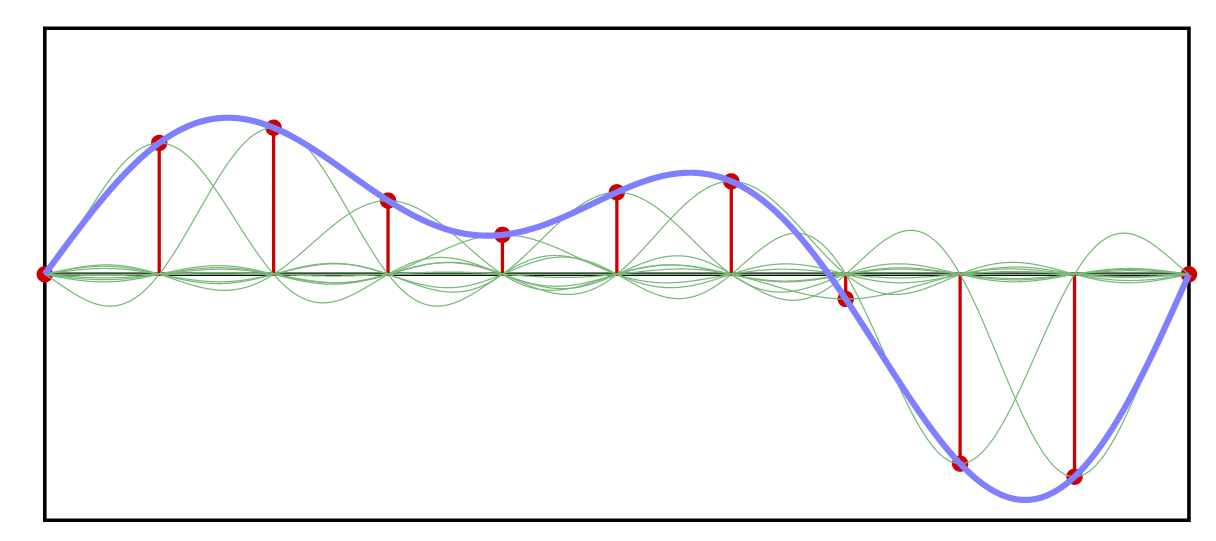
\includegraphics[scale=0.2]{images/sampling_theorem}
            \caption{Visualization of the sampling theorem}
            \label{fig:sampling_theorem}
        \end{figure}    
   
    \item[Discrete signal] Sequence of \textbf{complex} numbers. Notation: $x[n]$. $n$ is ``a-dimensional''. Analysis $\sim$ periodic measurements and Synthesis $\sim$ stream of generated samples.
    \item[Delta signal] $x[n] = \delta[n]$. 1 when $n=0$, 0 elsewhere.
    \item[Unit step] $x[n] = u[n]$. 1 when $n \geq 0$, 0 elsewhere.
    \item[Exponential decay] $x[n] = |a|^n u[n]$ with $|a| < 1$
    \item[Signal classes] Finite-length, infinite-length, periodic, finite-support
    \item[Finite-length] Notation: $x[n], n=0,1,...,N-1$. Vector: $\mathbf{x} = [x_0,x_1,...,x_{N-1}]^T$. Good for practice.
    \item[Infinite-length] Notation: $x[n], n\in\Z$. Abstraction $\to$ good for theory.
    \item[Periodic] N-periodic sequence $\tilde{x}[n] = \tilde{x}[n+kN],\quad k,n,N \in\Z$
    \item[Finite-support] $\overline{x}[n] = \left\{\begin{array}{ll}
    x[n] & \text{if} 0 \leq n < N\\
    0 & \text{otherwise}
\end{array}\right.$
    \item[Operators] \uline{Scaling}:$<y[n] = \alpha x[n]$. \uline{Sum}: $y[n] = x[n] + z[n]$. \uline{Product}: $y[n] = x[n]\cdot z[n]$. \uline{Shift by $k$} (delay): $y[n] = x[n-k]$
    \item[Finite-length shift] We must chose either to use \textit{finite-support} (0's outside of the interval, shifting ``creates'' 0's) or \textit{periodic extension} (leaving on a sides makes entering on the other).
    \item[Energy] 
        \begin{equation}
            E_x = \somme{\infty}{n=-\infty}|x[n]|^2
        \end{equation}
        Infinite for periodic signals
    \item[Power]
        \begin{equation}
            P_x = \limite{N\to\infty} \frac{1}{2N+1}\somme{N}{n=-N}|x[n]|^2
        \end{equation}
        For periodic signals: $P_{\tilde{x}} \equiv \frac{1}{N}\somme{N-1}{n=0}|\tilde{x}[n]|^2$
    \item[Legos] DPS is composed of fundamental building blocks. See figure \ref{fig:dsp_legos}.
        \begin{figure}
            \centering
            \begin{subfigure}{0.45\textwidth}
                \centering
                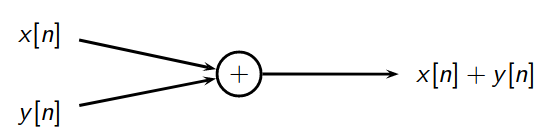
\includegraphics[scale=0.3]{images/lego_adder}
                \label{subfig:adder}
                \caption{Adder}
            \end{subfigure}
            \begin{subfigure}{0.45\textwidth}
                \centering
                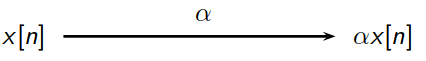
\includegraphics[scale=0.3]{images/lego_multi}
                \label{subfig:multi}
                \caption{Multiplier}
            \end{subfigure}\\
            \begin{subfigure}{0.4\textwidth}
                \centering
                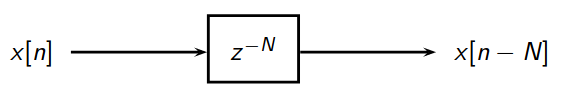
\includegraphics[scale=0.3]{images/lego_delay}
                \label{subfig:delay}
                \caption{N-delay}
            \end{subfigure}
            \begin{subfigure}{0.45\textwidth}
                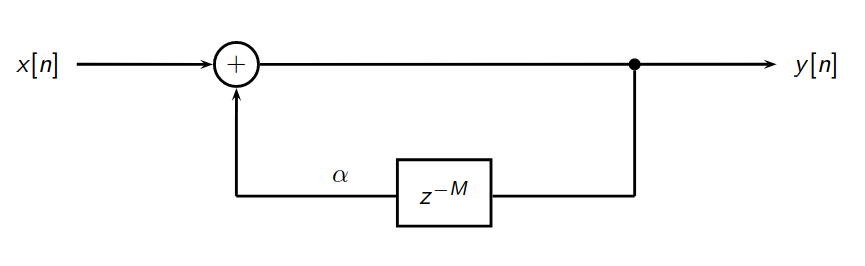
\includegraphics[scale=0.2]{images/loops}
                \caption{A looping system}
                \label{subfig:loop}
            \end{subfigure}  
            \caption{Fundamental building blocks}            
            \label{fig:dsp_legos}
        \end{figure}
  
    \item[Averages] Simple average: $m = \frac{a+b}{2}$. Moving average: take a ``local'' average 
        \begin{equation}
            y[n] = \frac{x[n] + x[n-1]}{2}
        \end{equation}
    \item[Loops]When feeding the output of a system to the input, we obtain a loop, of the type $y[n] = \alpha y[n-M] + x[n]$. This is a powerful concept ! Figure \ref{subfig:loop} shows an example. The parameters we can tweak: $M$ (size of delay), $\alpha$ (decay factor), $\overline{x}[n]$ (input signal)     
    \item[Karplus-Strong]\todo{}
\end{itemize}
\section{Vector spaces}
\begin{itemize}[font=\bfseries\uline]
    \item[Signal model]We work in $\C^N$: vector space  of ordered tuples of $N$ complex values. $N$ can be $\infty$. We need more than a vector space, we need a \textit{Hilbert space}.
    \item[Some spaces] $\ell_2(\Z)$: space of square-summable infinite sequences. $L_2([a,b])$: space of square-integrable functions over an interval
    \item[Vector spaces]Ingredients: the set of vectors $V$, and a set of scalars (say \C). We need at least to be able to: resize vectors (multiply vector by scalar) and combine vectors together (sum them).
    \item[Formal Properties]For $\mathbf{x},\mathbf{y},\mathbf{z} \in V$ and $\alpha,\beta \in \C$:
        \begin{multicols}{2}
            \begin{itemize}
                \item $\mathbf{x}+\mathbf{y} = \mathbf{y}+\mathbf{x}$
                \item $(\mathbf{x}+\mathbf{y}) + \mathbf{z} = \mathbf{x}+(\mathbf{x}+\mathbf{y})$
                \item $\alpha(\mathbf{x}+\mathbf{y}) = \alpha\mathbf{x} + \alpha\mathbf{y}$
                \item $(\alpha+ \beta)\mathbf{x} = \alpha\mathbf{x} + \beta\mathbf{x}$
                \item $\alpha(\beta\mathbf{x}) = (\alpha\beta)\mathbf{x}$
                \item $\exists 0 \in V | \mathbf{x} + 0 = 0+\mathbf{x} = \mathbf{x}$
                \item $\forall \mathbf{x} \in V \exists(-\mathbf{x}) | x+(- \mathbf{x}) = 0$
            \end{itemize}
        \end{multicols}
    \item[Dot Product]We also need something to measure and compare: \textbf{inner product} (or \textbf{dot product}). Notation: 
        \[\langle\cdot,\cdot\rangle : V\times V \to \C\]
        Measures similarity between vectors. If 0, then vectors are completely orthogonal.
    \item[Formal Properties]The dot product has several interesting properties. For $\mathbf{x},\mathbf{y},\mathbf{z} \in V$ and $\alpha\in\C$ :
    \begin{multicols}{2}
        \begin{itemize}
            \item $\langle\mathbf{x}+\mathbf{y},\mathbf{z}\rangle = \langle\mathbf{x},\mathbf{z}\rangle + \langle\mathbf{y},\mathbf{z}\rangle$
            \item $\langle\mathbf{x},\mathbf{y}\rangle = \langle\mathbf{y},\mathbf{x}\rangle^*$
            \item $\langle\alpha\mathbf{x},\mathbf{y}\rangle = \alpha^*\langle\mathbf{x},\mathbf{y}\rangle$\\
            $\langle\mathbf{x},\alpha\mathbf{y}\rangle = \alpha\langle\mathbf{x},\mathbf{y}\rangle$
            \item $\langle\mathbf{x},\mathbf{x}\rangle \geq 0$
            \item $\langle\mathbf{x},\mathbf{x}\rangle = 0 \iff \mathbf{x} = \mathbf{0}$
            \item If $\langle\mathbf{x},\mathbf{y}\rangle = 0$ and $\mathbf{x,y} \neq \mathbf{0}$ then $\mathbf{x}$ and $\mathbf{y}$ are orthogonal
            \item $\langle\mathbf{x},\mathbf{x}\rangle = ||\mathbf{x}||^2$
\end{itemize}
\end{multicols}
\end{itemize}

\end{document}